\section{Methodology}
\label{sec:methodology}

In this section, we first provide a functional example of a partial evaluation optimization. Then, we describe our implementation of partial evaluation in LLVM.

\subsection{Motivating Example}
\label{sec:motivatingexample}
Partial evaluation aims to specialize programs with respect to known inputs.
A number of partial evaluation techniques exist.
One variant of partial evaluation involves substituting function calls with constants, by evaluating branch and loop conditions with known program inputs.
This simplified approach was presented by Fujita’s work on partial evaluations~\cite{Fujita}.
If function calls can be replaced with constants, this reduces executable code, removes interactions with the call stack and avoids handling function return addresses.
This approach can also be implemented online at compile time.

Consider the following program in Figure~\ref{fig:original_sum}.
This program computes the sum of the arithmetic series, ending at the number $N$.

\begin{figure}[htbp]\
\begin{Verbatim}[frame=single,fontsize={\scriptsize},numbers=left,numbersep=5pt,xleftmargin=10pt]
int sum(int N)
{
  int i;
  int s = 0;
  for(i = 1; i <= N; ++i) {
    s += i;
  }
  return s;
}

int sum2(int N)
{
  return N*(N+1)/2;
}

int main(int argc, char **argv)
{
  int N = atoi(argv[1]);
  int gold = sum2(N);
  int s = sum(N);

  if(s != gold) {
    return 2;
  }

  printf("Success: sum(%d) = %d\n", N, s);
  return 0;
}
\end{Verbatim}
\caption{Original implementation of the sum program.}
\label{fig:original_sum}
\end{figure}

The program accepts one argument, $N$ as its input.
Suppose the input to this program is known such that $N = 6$. 
This can be the case for repetitive computations. 

First, line 18 can be substituted with $N = 6$.
If N is a constant, then the function call to \inlinecode{sum2()} at line 19 can be replaced with \inlinecode{gold = 21}.
This is obtained by evaluating \inlinecode{sum2()} with respect to the known value of $N$, which is $1 + 2 + ... + 6 = 21$ in this case. 
Similarly, the function call to \inlinecode{sum()} at line 20 can be replaced with \inlinecode{s = 21}.
Furthermore, the predicate block beginning on line 22 can be eliminated since $s = gold = 21$.
The resulting partial evaluation is shown in Figure~\ref{fig:pe_sum}.
Given the input to the this program, we were able to remove 2 function calls, and a predicate block.

\begin{figure}[htbp]\
\begin{Verbatim}[frame=single,fontsize={\scriptsize},numbers=left,numbersep=5pt,xleftmargin=10pt]
int main(int argc, char **argv)
{
  int N = 6;
  int s = 21;

  printf("Success: sum(%d) = %d\n", N, s);
  return 0;
}
\end{Verbatim}
\caption{Partial evaluation of the sum program for N=6.}
\label{fig:pe_sum}
\end{figure}

\subsection{Approach}

We implement the partial evaluation optimization as a transformation module pass in LLVM.
C/C++ programs are compiled to LLVM intermediate representation (IR) using the Clang front-end and the partial evaluation optimization pass is applied subsequently on the generated IR.

\begin{figure}[htbp]
  \centering
  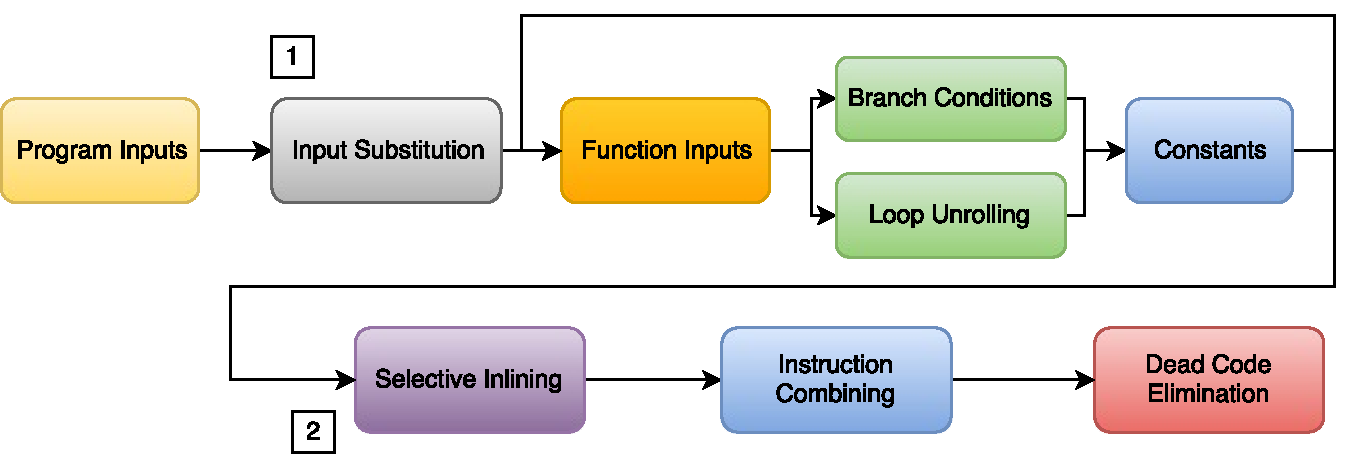
\includegraphics[keepaspectratio=true,width=\columnwidth]{PE_Diagram}
  \caption{Flow Chart of Online Partial Evaluation Optimization}
  \label{fig:pe_diagram}
\end{figure}

As observed in Section~\ref{sec:motivatingexample}, statically known program inputs can be leveraged towards reducing execution instructions. 
Hence, the optimization pass commences by substituting program variables with program inputs.
After variables are substituted with inputs, each function call is statically evaluated to eliminate branch conditions and loops.
Successfully reduced function calls can be safely converted to constants, while nested function calls will require the process to be repeated iteratively. 
Upon completion of this step, functions can be selectively inlined into the program.
Inlining eliminates the function call and integrates the remaining function instructions directly with the main program.
Instead of inlining every function in the program, we only inline functions that have been successfully reduced to constant operations.
Finally, any outstanding redundant instructions and dead code is eliminated.
A system diagram of our partial evaluation optimizer is shown in Figure~\ref{fig:pe_diagram}.

Adhering to the design principle, \textit{Separation of Concerns}, we opted to implement the minimal features required and allow subsequent passes to perform the rest of the optimization.
Since the default build of LLVM provides transformation passes to carry out constant propagation, loop unrolling, instruction combining and dead code elimination, we only need to develop the features of input substitution (1) and selective inlining (2) as marked in Figure~\ref{fig:pe_diagram}.

\bigbreak
\subsubsection{Input Substitution}

To perform input substitution, the optimization pass reads the program inputs from a user-defined input file. 
This is specified through a command line argument to the LLVM pass. 
The program inputs are substituted into variables referencing either the \inlinecode{argv} command line argument array or \inlinecode{fread()} instructions.
Candidate variables for input substitution include both local and global variables.

We provide an example of input substitution using the sum program.
Figure~\ref{fig:original_ir} displays the LLVM IR of the original, unoptimized sum program.

\begin{figure}[htbp]\
\begin{Verbatim}[frame=single,fontsize={\scriptsize},numbers=left,numbersep=5pt,xleftmargin=10pt]
define i32 @main(i32 %argc, i8** %argv) #0 {
...
  %11 = load i8**, i8*** %3, align 8
  %12 = getelementptr inbounds i8*, i8** %11, i64 1
  %13 = load i8*, i8** %12, align 8
  %14 = call i32 @atoi(i8* %13) #3
  store i32 %14, i32* %N, align 4
  %15 = load i32, i32* %N, align 4
  %16 = call i32 @sum2(i32 %15)
  store i32 %16, i32* %gold, align 4
  %17 = load i32, i32* %N, align 4
  %18 = call i32 @sum(i32 %17)
  store i32 %18, i32* %s, align 4
  %19 = load i32, i32* %s, align 4
  %20 = load i32, i32* %gold, align 4
  %21 = icmp ne i32 %19, %20
...
}
\end{Verbatim}
\caption{Original IR of the sum program.}
\label{fig:original_ir}
\end{figure}

Knowing that the variable N stores the input value 6, all instructions referring to \%N are replaced with 6.
The result of this optimization is shown in Figure~\ref{fig:input_sub_ir}. 

\begin{figure}[htbp]\
\begin{Verbatim}[frame=single,fontsize={\scriptsize},numbers=left,numbersep=5pt,xleftmargin=10pt]
define i32 @main(i32 %argc, i8** %argv) #0 {
...
  store i32 6, i32* %N, align 4
  %9 = call i32 @sum2(i32 6)
  store i32 %9, i32* %gold, align 4
  %10 = call i32 @sum(i32 6)
  store i32 %10, i32* %s, align 4
  %11 = load i32, i32* %gold, align 4
  %12 = icmp eq i32 %10, %11
...
}
\end{Verbatim}
\caption{Input substitution on the sum program, $N=6$.}
\label{fig:input_sub_ir}
\end{figure}

\bigbreak

\subsubsection{Selective Inlining}

LLVM provides a default function inlining transformation pass.
This default pass, however, inlines every function in the program.
In contrast, our optimization pass only inlines functions with constant instructions.
For example, if we encounter an instruction such as \inlinecode{\%x = add i32 1, \%y} in the function and \inlinecode{\%y} is not known, we will not inline the function.
As a result, our optimization pass will only eliminate function calls that are fully specialized to the program inputs.
While selective inlining does not alter the program behaviour, the program is able to retain function calls in unspecialized regions of the code.
It is important to retain such function calls to avoid erroneous partial evaluations, owing to poor variable visibility.

An example of selective inlining is shown in Figure~\ref{fig:inlining_ir}.
This example builds on top of the optimized IR, previously shown in Figure~\ref{fig:input_sub_ir}.
In this example, the function calls to \inlinecode{sum2()} and \inlinecode{sum()} are successfully inlined with the main function and replaced with constants.
The N variable is no longer needed by the program and is removed as a dead instruction.

\begin{figure}[htbp]\
\begin{Verbatim}[frame=single,fontsize={\scriptsize},numbers=left,numbersep=5pt,xleftmargin=10pt]
define i32 @main(i32 %argc, i8** %argv) #0 {
...
  store i32 21, i32* %gold, align 4
  store i32 21, i32* %s, align 4
  %5 = icmp eq i32 %gold, %s
...
}
\end{Verbatim}
\caption{Selective inlining on the sum program, $N=6$.}
\label{fig:inlining_ir}
\end{figure}

For the remainder of this paper, partial evaluation refers to our custom implementation on LLVM. 


\subsection{Fault Tolerance in Partial Evaluations}

Comparing the partial evaluation shown in Figure~\ref{fig:inlining_ir} with the original code in Figure~\ref{fig:original_ir}, the number of instructions have been significantly reduced.
We also notice that the partial evaluation can be further optimized by eliminating the \inlinecode{icmp} instruction and other subsequent dead blocks.
Despite the elimination of intermediary steps, the partial evaluation behaves exactly the same as the original program under normal conditions. 

Now, consider the scenario where an unexpected fault corrupts the value of \inlinecode{\%s}. 
In Figure~\ref{fig:inlining_ir}, the program will be able to detect the corruption of \inlinecode{\%s} through the compare instruction on line 5.
However, if the compare instruction is eliminated through additional optimizations, the program will not be able to detect this corruption in the same basic block.
This would allow the error to propagate further down the optimized program than the original program.
This scenario could lead to a deterioration of error resilience if the corrupted variable is referenced in subsequent instructions. 
